\chapter{Contribution to the DREAM project} \label{app:dream}

As part of DREAM, I have been involved in various meetings, developed tools to automate tasks and contributed to a significant part of the software developed during the project.

\section{Software development}

WP6, composed of Plymouth and VUB, was responsible to develop the cognitive controller of the robot. I developed mostly alone the deliberative, expression and actuation and naoInterface subsystems. I also converted scripts provided by the therapist into steps the robot can follow and programmed a robot behaviour corresponding to each one of these steps.


\section{Tools}

In addition to the components developed to run the DREAM application, I created two tools to automate and simplify the use of the YARP middleware while conforming to the development standards imposed on the project.

\subsection{yarpGenerator}

The software development guidelines of DREAM imposed a specific structure for folders of new components developed with a number of constant part throughout the required 6 files. Additionally, adding or removing one port required changes in 5 files in more than 10 location. To ease this procedure, I proposed to add two new class: the yarpInterface and the yarpController. yarpInterface class exposes all the yarp output port required by the component to C++ function and integrates function asynchronously called when messages arrive on input ports. And the yarpController corresponds to a C++ only file where the code can be developed without reliance of YARP. This class (and others) can call functions from yarpInterface to send messages and be called by callbacks in yarpInterface to react to messages. The yarpGenerator is a tool generating automatically compilable code, complient with the development standards. Appendice B presents the techreport created to describe the tool.

\subsection{scriptManager}

The second tools aims at providing a graphical way to read and edit the xml files describing the scripts used in the therapies.

\cleartooddpage
\chapter{State Space Used for Tutoring Study} \label{app:state}
\begin{table}[ht]
	\centering
	\ra{1.2}
	\caption{Definition of each category of the state space.}
	\label{tab:tutoring_policies}
	\begin{tabularx}{\textwidth}{@{}llX@{}}\toprule
		Name & Number & Description \\
		\midrule
		Distance between items & 155 & Normalised distance between the animals and each other animal and the plants\\
		Items' energy & 21 & Energy of the 21 items(10 animals and 11 plants)\\
		Time since robot touches & 10 & Time since the robot touched each animal\\ %decay
		Time since child touches & 10 & Time since the child touched each animal\\ %accumulation
		Progress in the game & 1 & 0.25 for 1st game to 1 for the last game\\ 
		Generic events & 3 & Time since last feeding, failed interaction and death of an animal\\ %decay
		Last robot's actions & 5 & Time since last type of robot action\\ %decay
		Generic last action & 2 & Time since any child touch and robot action\\ %decay\accumulation
		Focus & 3 & Value of focus toward the robot, the screen and outside\\ %accumulation
		\bottomrule
	\end{tabularx}
\end{table}

To compute time, two methods have been used:
\begin{itemize}
	\item Accumulation: for the times since child touches and focus (effect being true or false).
	\item Decay: for robot actions and touches and generic events (discrete events).
\end{itemize}

When the effect is true for accumulation, the state value is set to 0.5 and increases each step (by $1-e^{-\frac{1}{10}}$ of the missing value). And when the condition is false, the value is set to 0.5 and decreases (by being multiplied by $e^{-\frac{1}{10}})$. Similarly for the decay, when the event happens the value is set to 1 and then exponentially decreases by being multiplied by $e^{-\frac{1}{10}}$. That way event will have a `half-life' of 7 steps, which corresponds to 3.5 seconds.

Each instance of a plant is considered as a unique element. For example, there are four instances of wheat, however each one is considered uniquely as a non-moving image. It could have been possible to group the instances by categories, but it would require some add-hoc coding, limiting the generalisation of the approach.

\cleartooddpage
\chapter{Action Space Used for Tutoring Study} \label{app:action}
\begin{table}[ht]
	\centering
	\ra{1.2}
	\caption{Definition of each category of the action space.}
	\label{tab:tutoring_policies}
	\begin{tabularx}{\textwidth}{@{}llX@{}}\toprule
		Name & Number & Description \\
		\midrule
			Move close & 210 &  Action moving any animal close to any item\\
			Move to & 210 & Action moving any animal to any item\\
			Move away & 210 & Action moving any animal away from any item\\
			Remind rules & 1 & \\
			Congratulation & 1 & \\
			Attention & 21 & Drawing attention to any item\\
			Encouragement & 1 & \\
			Wait & 1 & Doing nothing\\
		\bottomrule
	\end{tabularx}
\end{table}

The total action space available is 655 actions. It should be noted that technically 30 actions exist but cannot be selected by the teacher (moving animals to/close to/away from themselves). But this does not impact the learning as an instance based algorithm is used. Similarly to the states, each instances of a same category (such the different images of the wheat) is considered as a unique non-moving item to create actions.


\cleartooddpage
\chapter{Teacher's Diary} \label{app:diary}
This appendix section present the daily report of the teacher's impressions and feeling when teaching the robot in the study in Chapter\ref{chap:tutoring}. It should be noted that among all the children supervised, many were special needs and as such have been removed from the result analysis. This also explains the difference of number between the children in the supervised condition (n=25) and in this diary (n=34).

%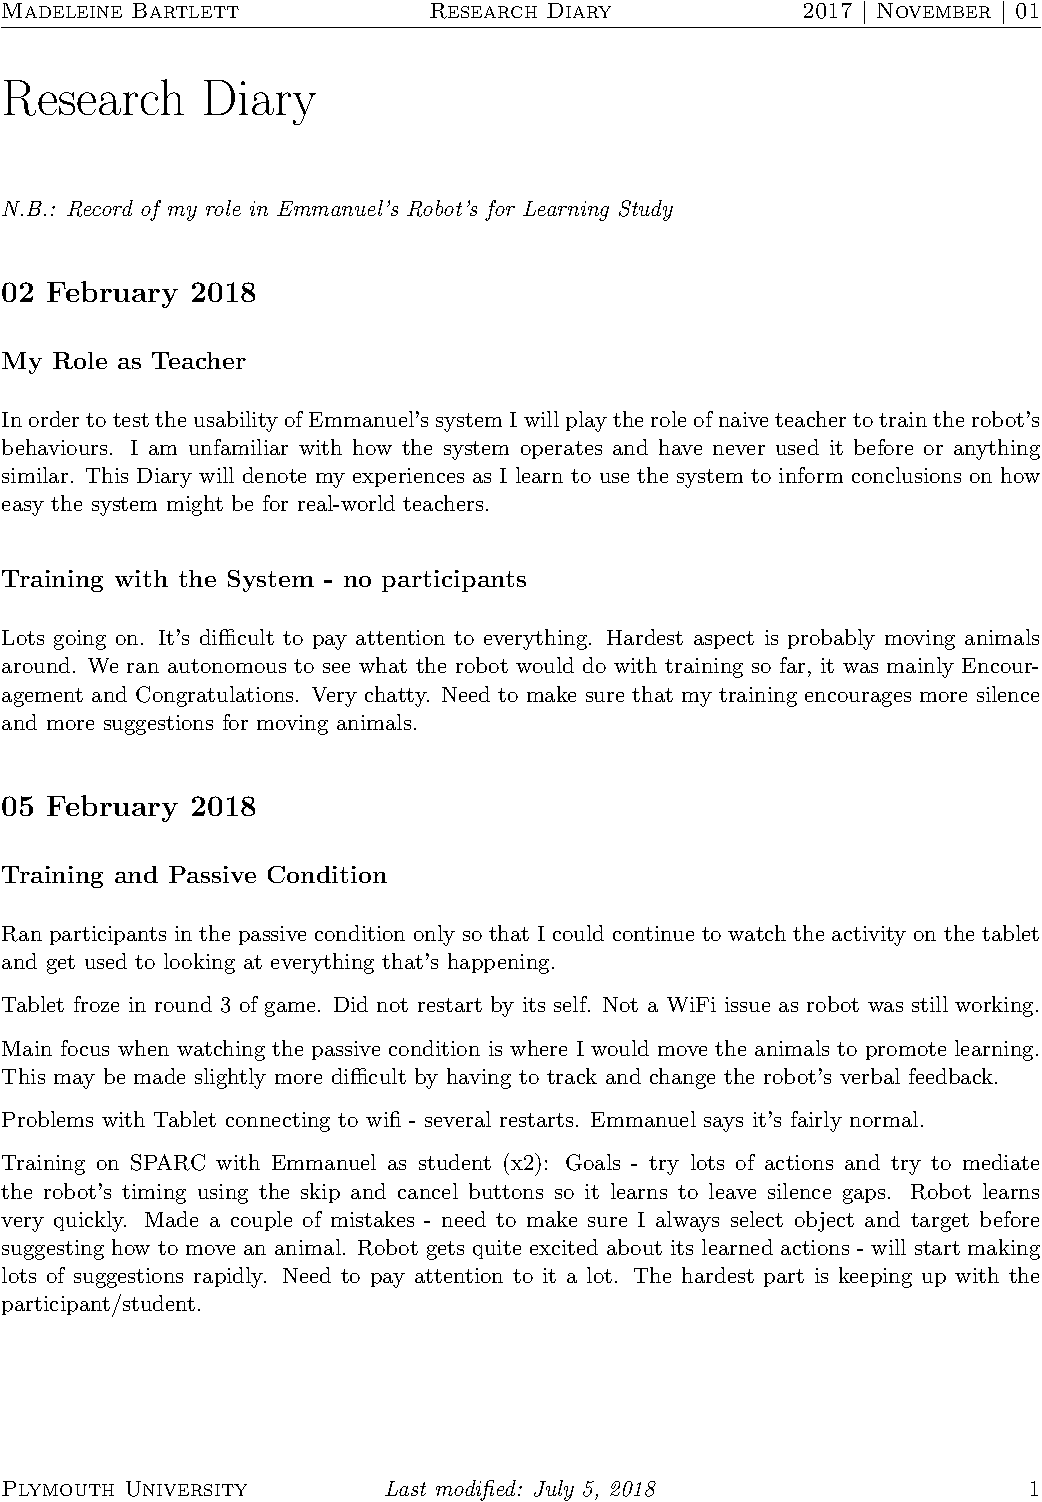
\includepdf[pages=1-14,pagecommand={},linktodoc=true]{appendices/research-diary.pdf}
\foreachpage{appendices/research-diary-crop.pdf}{%
	\newpage   
	\begingroup 
	\centering
	\includegraphics[
	page=\value{imagepage},
	width=\textwidth,  
	height=\textheight,
	keepaspectratio,
	]{appendices/research-diary-crop.pdf}%
	\newpage
	\endgroup
}